

\begin{figure}[ht]
\centering
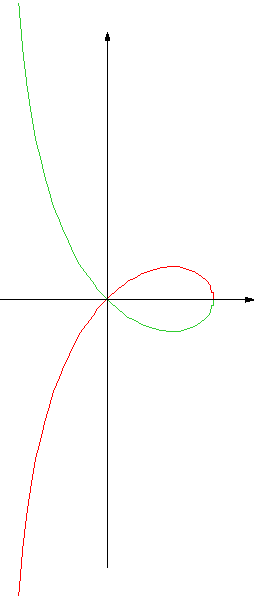
\includegraphics{Cgep4_1.pdf}
\caption{Courbe $\mathcal C$}
\label{fig:Cgep4_1}
\end{figure}
\begin{enumerate}
\item  Soit $M$ de coordonn{\'e}es$(x,y)$, un point quelconque du plan. Ce point est dans $\mathcal{P}$ si et
seulement si il existe $B_{t}$ de coordonn{\'e}es $(0,t)$ v{\'e}rifiant les conditions impos{\'e}es soit :
\[
(S)\quad \left\{
\begin{array}{c}
x^{2}+(y-t)^{2}=16\quad \quad \quad (1) \\
x(x-4)+(y-t)y=0\quad (2)
\end{array}
\right.
\]
Supposons $y\neq 0$ c'est {\`a} dire que $M$ n'est pas sur l'axe des $x$. On a alors
\[
(S)\Leftrightarrow \left\{
\begin{array}{c}
(1) \\
y-t=\frac{x}{y}(4-x)
\end{array}
\right. \Leftrightarrow \left\{
\begin{array}{c}
y-t=\frac{x}{y}(4-x)\quad \quad \quad (1^{\prime }) \\
x^{2}+\frac{x^{2}}{y^{2}}(4-x)^{2}=16\quad (2^{\prime })
\end{array}
\right.
\]
\[
(2^{\prime })\Leftrightarrow (x-4)(x+4+\frac{x^{2}}{y^{2}}%
(4-x))=0\Leftrightarrow (x-4)(y^{2}(x+4)+x^{2}(4-x))=0
\]
Lorsque $M$ est sur l'axe des $x$, le syst{\`e}me $(S)$ devient
\[
\left\{
\begin{array}{c}
x^{2}+t^{2}=16 \\
x(x-4)=0
\end{array}
\right.
\]
On en d{\'e}duit que l'intersection de $\mathcal{P}$ avec l'axe des $x$ est form{\'e} par l'origine et $A$. Finalement, $\mathcal{P}$ est l'union de la droite $\mathcal{D}$ d'{\'e}quation $x=4$ et de la courbe $\mathcal{C}$ d'{\'e}quation
\[
y^{2}(x+4)+x^{2}(4-x)=0
\]
Si $(x,y)$ v{\'e}rifie cette {\'e}quation, $(x,-y)$ la v{\'e}rifie aussi. La courbe $\mathcal{C}$ est sym{\'e}trique par rapport {\`a} l'axe des $x$.

\item La courbe $\mathcal{C}$ est l'union des graphes de $f$ et de $-f$ o{\`u} $f$ est d{\'e}fini par
\[
f(x)=x\sqrt{\frac{4-x}{4+x}}\text{, }x\in \left] -4,4\right[
\]
Apr{\`e}s calculs, on obtient 
\begin{displaymath}
 f'(x)=\dfrac{20-(x+2)^{2}}{\sqrt{4-x^{2}}}
\end{displaymath}
La fonction est croissante de $-4$ {\`a} $2(\sqrt{5}-1)$ puis d{\'e}croissante.\newline
Au voisinage de $-4$, le graphe admet la droite d'{\'e}quation $x=-4$ comme asymptote. Au voisinage de 4, il admet $A$ comme point limite avec une tangente verticale. Voir figure \ref{fig:Cgep4_1}

\item  L'{\'e}quation de la courbe $\mathcal{C}-\{O\}$ s'{\'e}crit encore
\[
x+4+\left( \frac{x}{y}\right) ^{2}(x-4)=0\Leftrightarrow x(1+\left( \frac{x}{%
y}\right) ^{2})=4(1-\left( \frac{x}{y}\right) ^{2})
\]
En posant $t=\frac{x}{y}$, on en d{\'e}duit que $\mathcal{C}-\{O\}$
est l'ensemble des $M(t)$ lorsque $t$ est diff{\'e}rent de 1 et de
$-1$. De plus $O=M(-1)=M(1)$. L'origine est le seul point double
de cette courbe param{\'e}tr{\'e}e.
\item \begin{enumerate}
 \item Soit $C=M(p)$ l'intersection de $\mathcal{P}$ avec la droite d'{\'e}quation $x-py=0$. La droite
d'{\'e}quation $px+y=0$ est orthogonale {\`a} la premi{\`e}re. Son intersection avec $\mathcal{P}$ est $D=M(-\frac{1}{p})$. Comme $M(-\frac{1}{p})$ {\`a} pour coordonn{\'e}es
\[
(-4\frac{1-p^{2}}{1+p^{2}},\frac{4}{p}\frac{1-p^{2}}{1+p^{2}})
\]
les coordonn{\'e}es de $\overrightarrow{M(-\frac{1}{p})M(p)}$ sont donc
\[
(8\frac{1-p^{2}}{1+p^{2}},4(p-\frac{1}{p})\frac{1-p^{2}}{1+p^{2}})=\frac{4}{p%
}\frac{1-p^{2}}{1+p^{2}}(2p,p^{2}-1)
\]
L'{\'e}quation de $(CD)$ est $(p^{2}-1)x-2py+4(1-p^{2})=0$.

\item  Ordonnons l'{\'e}quation de $(CD)$  suivant les puissances de $p$ 
\[
(x-4)p^{2}-2py+4(1-p^{2})=0
\]
On en d{\'e}duit que toutes les droites $(CD)$ passent par le point $A$.
\end{enumerate}
\item Soit $\mathcal{D}$ une droite passant par l'origine, $\mathcal{D}^{\prime }$ sa sym{\'e}trique par rapport {\`a} la premi{\`e}re bissectrice.\newline
On suppose que $\mathcal{D}$ n'est ni un des axes ni une des bissectrices. Dans ce cas, les {\'e}quations de $\mathcal{D}$ et $\mathcal{D}^{\prime }$ sont respectivement 
\begin{displaymath}
 y-px=0 \text{ et } x-py=0 \text{ avec } p\notin \{-1,0,1\}
\end{displaymath}
On a aussi $E=\mathcal{D}\cap \mathcal{C}=M(\frac{1}{p})$, $F=\mathcal{D}^{\prime }\cap \mathcal{C}=M(p)$. Les coordonn{\'e}es de $M(\frac{1}{p})$ sont
\[
(-4\frac{1-p^{2}}{1+p^{2}},-4\frac{1}{p}\frac{1-p^{2}}{1+p^{2}})
\]
On en d{\'e}duit que $\overrightarrow{M(\frac{1}{p})M(p)}$ est colin{\'e}aire {\`a} $(1,\frac{1}{2}(p+\frac{1}{p}))$. L'{\'e}quation de la droite $(EF)$ est alors
\[
(p^{2}+1)x-2py=4\frac{(1-p^{2})^{2}}{1+p^{2}}
\] 

\end{enumerate}
